% !TeX encoding = UTF-8
% !TeX spellcheck = it_IT
% !TEX root = main.tex

\chapter{Cos'è un algoritmo? Definizione e qualche esempio}
Cos'è un algoritmo? Eh, domanda non troppo facile ma senz'altro di fondamentale importanza. Ormai siamo nell'era digitale, dove gli algoritmi regano sovrani. Tutti i dispositivi che utilizziamo quotidianamente sono basati su essi, direi quindi che un po' di loro conoscenza non guasta a nessuno ;) .Cos'è un algoritmo?

\section{Introduzione ed esempi pratici}

Per definire questo "oggetto", vediamo di partire da un semplice esempio ;) Sai preparare la pasta giusto? Bene, mentre la prepari segui un algoritmo ben preciso:

\begin{enumerate}
	\item Metti l'acqua nella pentola
	\item Accendi il fuoco e sopra ci metti la pentola
	\item Aspetti 5-10 minuti che l'acqua bolla
	\item Pesi la pasta su una bilancia
	\item Aggiungi il sale all'acqua
	\item Aggiungi la pasta nella pentola
	\item Aspetti 5-10 minuti di cottura
	\item Al termine la scoli e la aggiungi al sugo.
	\item Quindi la servi nel piatto
\end{enumerate}

Chiaramente non fissiamoci troppo sui dettagli della preparazione della pasta, magari tu hai una ricetta super segreta diversa da questa ;) Comunque l'importante è rendersi conto che esistono delle istruzioni che vanno bene in qualsiasi momento per prepararla e funzionano sia che le metta in pratica io che tu. Inoltre il risultato è sempre lo stesso, un bel piattone di pasta 

Vediamo quindi di estrarre le proprietà fondamentali di un algoritmo a partire da questo semplice esempio. Esso è una sequenza di istruzioni/azioni che vanno eseguite in un ordine specifico. Questa sequenza è inoltre finita in tempo, nel senso che sai già che riuscirai a preparare il tuo piatto di pasta in 15-20 minuti. Inoltre questa ricetta non può essere ambigua, interpretabile, ma deve funzionare chiunque sia il "cuoco". Per concludere, le istruzioni devono essere elementari, semplici, non ulteriormente spezzabili in azioni più semplici.

Vediamo quindi un esempio più matematico prima di arrivare a definirli formalmente ;)

\subsection*{Algoritmo di Euclide}

É un algoritmo che si usa per trovare il massimo comun divisore tra due numeri naturali qualsiasi. Se non sai cosa sia il massimo comun divisore (MCD), è semplicemente il numero naturale più grande in grado di dividere esattamente i numeri di partenza. Quindi si ha che esso è uguale ad 1 nel caso essi siano coprimi, ovvero privi di divisori comuni.

Ecco l'algoritmo scritto in linguaggio comune (pseudocodice):

\begin{verbatim}
	Prendi a,b numeri naturali
	Definisci una variabile naturale r
	Finchè b diverso da 0 :
		r = a % b (il resto della divisione tra a e b)
		a = b
		b = r 
	
	Restituisci a
\end{verbatim}

Ora non sto qui troppo a soffermarmi sul perchè questo algoritmo funzioni, magari dai una letta qui ALGORITMO MCD DI EUCLIDE, qualche spunto interessante lo troverai di sicuro ;)

Ciò che importa  per il nostro obiettivo attuale è notare come le operazioni che questo algoritmo comporta sono elementari: divisioni intere e sostituzioni di variabili, niente di più.

Inoltre questo algoritmo fa al più $ b $ iterazioni del ciclo, nel caso in cui essi siano coprimi e quindi termina in tempo finito :) Proprio come avevamo notato prima nell'algoritmo per la pasta.

Chiaramente questo è un algoritmo ancora semplice, in fondo all'articolo ti indicherò alcuni algoritmi grossi e importanti così da farti venire voglia di approfondire l'argomento da solo ;)

\section{Definizione più rigorosa del concetto di \textit{algoritmo}}

\begin{defn}
	Si dice algoritmo una sequenza finita e ordinata di operazioni elementari e non ambigue che permettono di risolvere, in maniera deterministica, un problema in tempo finito, ovvero l'algoritmo ha un termine.
\end{defn}

Se non hai mai sentito parlare di algoritmo in termini un po' più formali, è molto probabile che ti sfugga l'importanza di qualcuna delle richieste che l'algoritmo deve soddisfare per essere definito tale.

Vediamo quindi un paio di esempi che sembrerebbero algoritmi ma non lo sono perchè non rispettano una o più di queste strane proprietà.

Un esempio semplice di non determinismo di una sequenza di istruzioni potrebbe essere introdotta nella procedura di preparazione della pasta. Per esempio si decide che appena si è messa l'acqua a bollire si lancia un dado e a seconda del numero che esce si salterà una delle operazioni che abbiamo elencato successivamente. Non solo questa procedura non è deterministica ma non è nemmeno detto che ci permetta di ottenere il risultato finito :)

Un altro "algoritmo" molto semplice ma che non può essere definito tale in quanto non termina è il seguente:

\begin{verbatim}
	a = 2

Finchè a è pari:

a = 2a

Restituisci a
\end{verbatim}
Chiramente se moltiplichiamo un numero pari per 2, esso rimarrà pari ;) Può sembrare stupido come esempio, ma è sufficientemente chiaro per capire l'importanza di queste proprietà nella buona caratterizzazione di un algoritmo.

Per finire questa carrellata di esempi di non algoritmi, discutiamo un attimo della non ambiguità. Un esempio molto semplice, legato per sempre alla preparazione della pasta, è il seguente:

Nella ricetta invece di dire dopo 10 minuti spegni il fuoco e scola la pasta, supponi di dire di scolarla quando ti sembra cotta.

Il "sembrare cotta" non è chiaramente un parametro oggettivo. Sono d'accordo che nella realtà lo si dice, ma non è un problema dato che noi non siamo macchine ma uomini e donne pensanti, in grado di fare delle scelte in autonomia. Però se si dicesse così ad un computer, o comunque dare queste istruzioni ad una planetaria o un robottino che cucina per te, è ovvio che lui non sarebbe in grado di decidere quando scolare la pasta (a meno di insegnarglielo, ma questo è un discorso più complicato) ;) Ecco il perchè dell'importanza della non ambiguità delle istruzioni.

Proprio perchè queste proprietà devono appartenere ad un qualsiasi algoritmo, essi sono anche rappresentabili mediante un diagramma di flusso. Qui sotto ti allego una immagine tipo e in un altro articolo magari approfondiremo la visione grafica degli algoritmi...merita davvero più spazio che qualche riga stracciata qui.

\begin{figure*}
	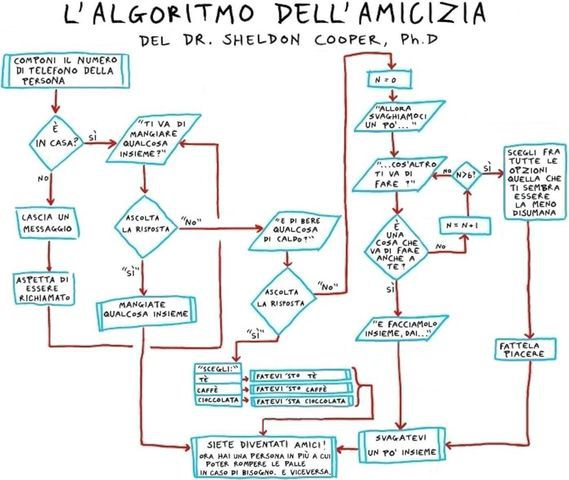
\includegraphics[width=\textwidth]{amicizia}
	\caption{Fonte dell'immagine: Nonciclopedia}
\end{figure*}

Prima di concludere l'articolo, ti lascio un elenco con alcuni algoritmi interessanti a cui ti consiglio di dare un'occhiata. Se c'è interesse, magari ne approfondiremo qualcuno nei prossimi articoli, in caso faccelo sapere mandando un messaggio alla Pagina Facebook, lasciando un commento qui sotto al post o mandando una mail all'indirizzo list@mathone.it :)

\section{Alcuni algoritmi interessanti da approfondire}

Preferisco sviluppare questa sezione in maniera molto schematica, lasciandoti una semplice lista di link che rimandano ad una pagina di approfondimento dedicata al particolare algoritmo, per parlarne sul sito ci sarà tempo in futuro :)

\begin{itemize}
	\item Algoritmo di ricerca di Google
	\item Algoritmi di ordinamento
	\item Algoritmo di Dijkstra (distanza minima)
	\item Algoritmi di raccomandazione
	\item Algoritmi di compressione dati senza perdita
\end{itemize}

Ce ne sarebbero molti altri ma per ora direi che è una lista anche troppo lunga, se vuoi guardare qualcos'altro su questo sito, ecco alcuni articoli legati a queste tematiche che avevamo scritto in passato:

Algoritmo calcolo radice quadrata
Algoritmo moltiplicazione egizia
Alla scoperta di algoritmi antichi e curiosi